\documentclass[10pt]{siamltex}
% siamltex     final
\usepackage{amsmath,amssymb,epsfig}
\usepackage{listings}
%\usepackage[]{graphicx,epsf,epsfig,amsmath,amssymb,amsfonts,latexsym,amsthm}
% \usepackage{bbm}
%\usepackage{amsfonts}
%\usepackage{amsthm}
%% \usepackage[a4paper]{geometry}
%% \geometry{top=0.99in, bottom=0.995in, left=0.995in, right=0.995in}
% \usepackage[top=20mm, bottom=18mm, left=15mm, right=18mm]{geometry}
\usepackage[top=18mm, bottom=18mm, left=20mm, right=20mm]{geometry}

\usepackage{hyperref}

% \graphicspath{{/Users/Mihai/Google Drive/MATLAB/Ranking_Sync/PLOTS/}}
% D:/LATEX/Reports@IIT/figures/
\usepackage{graphicx}
\usepackage[space]{grffile}

\newcommand{\mb}[1]{\mbox{\boldmath$#1$}}

\usepackage{lineno}
\pagewiselinenumbers

\usepackage{subfigure}
\usepackage{amsmath}
\usepackage{amssymb}
\usepackage{graphicx}
\usepackage{comment}
\usepackage{array}
\usepackage{algorithm}
\usepackage{algorithmic}
\usepackage{url}
\usepackage[algo2e]{algorithm2e}
% \usepackage{color}

% \usepackage[toc,page]{appendix}

%\usepackage[outer]{showlabels,rotating}
%\renewcommand{\showlabelsetlabel}[1]
%{\begin{turn}{0}\showlabelfont #1\end{turn}}
%\showlabels{cite}
%\showlabels{ref}
%\showlabels{foo}
%\renewcommand{\showlabelfont}{\small}

\usepackage{setspace}
\usepackage{multicol}
\usepackage{multirow}
\usepackage{color}
\usepackage{colortbl}
\usepackage{xcolor}
\usepackage{hyperref}
%\def\Acronimo{ANALYSISOFNETWORKS}
% number the lines

\newcommand{\myreferences}{../../../Postdocs_laptop/postdoc_bib_file}
% \newcommand{\myreferences}{/Users/Mihai/test_bib_file}

\usepackage{lineno}
% \pagewiselinenumbers
%\setlength\linenumbersep{8pt}

% ANALYSISOFNETWORKS
% AALGN
\hypersetup{
%    pdftitle={\Acronimo{}, FP7-PEOPLE-IIF-2012},    % title
%    pdfauthor={Some Author},
    colorlinks=true,
    citecolor=red,
    linkcolor=blue,
    urlcolor=blue
  }

%
%\newtheorem{theorem}{Theorem}[section]
%\newtheorem{conjecture}[theorem]{Conjecture}
%\newtheorem{corollary}[theorem]{Corollary}
%\newtheorem{proposition}[theorem]{Proposition}
%\newtheorem{lemma}[theorem]{Lemma}
%\newdef{definition}[theorem]{Definition}
%\newdef{remark}[theorem]{Remark}
\newcounter{ale}
\newcommand{\abc}{\item[\alph{ale})]\stepcounter{ale}}
\newenvironment{liste}{\begin{itemize}}{\end{itemize}}
\newcommand{\aliste}{\begin{liste} \setcounter{ale}{1}}
\newcommand{\zliste}{\end{liste}}
\newenvironment{abcliste}{\aliste}{\zliste}

% \usepackage[english]{datetime}

\def\P(#1){\Phelper#1|\relax\Pchoice(#1)}
\def\Phelper#1|#2\relax{\ifx\relax#2\relax\def\Pchoice{\Pone}\else\def\Pchoice{\Ptwo}\fi}
\def\Pone(#1){\Pr\left( #1 \right)}
\def\Ptwo(#1|#2){\Pr\left( #1 \mid #2 \right)}
\def\Pr{\mathbf{Pr}}

\begin{document}

\begin{pagewiselinenumbers}
\title{MATH 191 - Topics in Data Science\\ Discovering Hidden Prerequisites}
\author{Paul~Jazayeri \footnotemark[1], Anumat~Srivastava \footnotemark[2], Lowell~Bander \footnotemark[3]  }
\maketitle
%\renewcommand{\thefootnote}{\fnsymbol{footnote}}
\footnotetext[1]{Department of Mathematics, UCLA, 520 Portola Plaza, Mathematical Sciences Building 6363, Los Angeles, CA 90095-1555}
\footnotetext[2]{Second Department, UCLA, 520 Portola Plaza, Mathematical Sciences Building 6363, Los Angeles, CA 90095-1555}
\footnotetext[3]{Computer Science Department, UCLA, 4732 Boelter Hall
Los Angeles, CA 90095}
%\renewcommand{\thefootnote}{\arabic{footnote}}

\begin{center}
\today
\end{center}

% We propose novel approach to the
\vspace{5mm}

\begin{abstract}
%Abstract goes here. Provide 10-15 lines with a summary of your work.
We sought to use historical student data to discover/validate the prerequisite choices of the Mathematics and Computer Science at the University of California, Los Angeles (UCLA). Specifically, we used the Serial Rank, Rank Centrality, and Least Squares ranking algorithms to construct total orderings of courses so as to optimize graduating grade-point average (GPA). We then implemented the Kednall Tau Distance algorithm to determine the degree with which our various ranking algorithms agreed in the total ordering they outputted. Finally, used intermediate calculations from the above ranking algorithms to construct a directed acyclic graph (DAG) to illustrate the notion of courses being prerequisites for other courses.
\end{abstract}

\begin{keywords} %A few keyword that best describe your work. For example:  network centrality, spectral algorithms, gravity models, vertex similarity, core periphery structure, directed graphs, local-to-global algorithms, multiple network alignment, clustering bipartite graphs, angular synchronization
serial rank, rank centrality, prerequisites, least squares, kendall tau distance
\end{keywords}

\section{Introduction}

The lecture on ranking algorithms was perhaps one of the most eye opening applications introduced in this course. As students, we have seen that courses are sometimes listed as prerequisites for other courses, when in fact they ought not to be. Conversely, we have seen that some courses perhaps should be prerequisites, given that one course serves as such a good primer for another and makes the subject matter much less daunting.\\

Because of this, we sought to use various ranking algorithms to empirically determine which courses should in fact be taken before other courses.\\

In Section \ref{sec:ourWork} we describe our attempts to acquire the requisite data for this report, and then go on to describe the algorithms we used on the data we acquired. In Section  \ref{sec:NumExpSyn} we test the above algorithms on synthetically generated data sets, while in Section \ref{sec:NumExpReal} we do so for a real data set. Finally, in Section  \ref{sec:conclusion} we conclude with a summary of our results, and discuss future possible research direction. 

\section{Related work} \label{sec:relWork}\textcolor{white}{.}\\

[1] Sedgewick, Robert. \textit{Algorithms}. Reading, MA: Addison-Wesley, 1988. Print. Chapter 2.5 Sorting Applications, Kendall tau distance.\\

[2] Negahban, Sahand, Sewoong Oh, and Devavrat Shah. ``Iterative Ranking from Pair-wise Comparisons." Advances in Neural Information Processing Systems 25 (2012): 2474-482. Http://papers.nips.cc/paper/4701-iterative-ranking-from-pair-wise-comparisons.pdf. Curran Associates, Inc. Web.\\

[3] Fogel, Fajwel, Alexandre D'Aspremont, and Milan Vojnovic. ``SerialRank: Spectral Ranking Using Seriation." SerialRank: Spectral Ranking Using Seriation (n.d.): n. pag. Web.\\

[4] Statistical Models Applied to the Rating of Sports Teams, Kenneth Massey\\

[5] Sync-Rank: Robust Ranking, Constrained Ranking And Rank Aggregation Via Eigenvector And Sdp Synchronization, Mihai Cucuringu

\section{Our work}    \label{sec:ourWork}
%Describe the bulk of your work in this section.
\subsection{Getting Started}
Our first steps in this endeavor involved acquisition of the data requisite to perform out analysis. Specifically, we sought to obtain, for several students, in both the Mathematics (Math) and Computer Science (CS) departments, over many years: (1) the order in which each student took their courses, and (2) their graduating GPA for the relevant department, either Math or CS.\\

Our professor for this course, Mihai Cucuringu, had previously obtained the requisite dataset from the Math department and was kind enough to share this with us. Unfortunately, we were not successful in obtaining the corresponding dataset for the CS department before the due date of this project. This is not for lack of effort, for we approached members of the Registrar's office, the current and a former chair of the CS department, as well as the Office of Academic and Student Affairs for the School of Engineering and Applied Science (OASA SEAS).\\

As mentioned in the abstract of our paper, we sought to implement various ranking algorithms to determine total orderings of courses as a method of validating existing prerequisites and potentially discovering hidden ones, courses that ought to be prerequisites but are not currently. Moreover, we sought to visualize the prerequisite relationship among courses by construction of a directed acyclic graph (DAG), wherein children nodes have parents as their prerequisites, and wherein the edge weights between nodes represents the confidence with which our data supports one course being a prerequisite for another course. \\

\subsection{Serial Rank}
As we began implementation of the Serial Rank algorithm we noted that an intermediate computation of the algorithm would prove very useful in the construction of the DAG described above. Namely, both share the need for a matrix $C$ containing pairwise comparisons, such that $C\in \{-1,0,1\}^{n\times n}$, where $n$ is the number of courses a student takes. The elements of $C$ are determined as follows:

\begin{equation}
C_{ij} = \left\{
	\begin{array}{rl}
 1 & \text{ if course $i$ is taken before course $j$, (or $i=j$)} 	\\
 &  \\
 0 & \text{ if $i$ and $j$ are tied, or the comparison is unavailable }	\\
 &  \\
 -1 & \text{ if course $j$ is taken before course $i$} 
     \end{array}
   \right.
\label{comparisonMatrix1}
\end{equation}
By convention we define $C_{i,i} = 1$ for all $i \in \{1, \dots, n\}$ ($C_{i,i}$ values have no effect in the
ranking method presented in algorithm SerialRank.\\
After constructing the comparison matrix $C$ we define the pair-wise similarity matrix $S^{\text{match}}$ as $$S^{\text{match}} = \sum_{k = 1}^{n} \frac{1+C_{ik}C_{j, k}}{2}$$
Thus $S^{\text{match}}_{ij}$ counts the number of matching comparisons between $i$ and $j$ with other reference
items $k$. Equivalently $S^{\text{match}}$ can be expressed in closed-form as $$S^{\text{match}} = \frac{1}{2}(n11^T + CC^T)$$
\begin{algorithm}[H]
\KwData{A set of pairwise comparisons $C_{i,j} \in \{1, 0, 1\}$ or $[1, 1]$.}
\begin{enumerate}
\item Compute the similarity matrix $S$ as described above
\item Compute Laplacian matrix $$L = D - S$$ where $D$ is a diagonal matrix and $D_{i, i} = \sum_{j = 1}^{n}S_{ij}$ is the degree of node $i$.
\item Compute the Fiedler vector of S.
\end{enumerate}
\KwResult{A ranking induced by sorting the Fiedler vector of $S$}
 \caption{Serial Rank Algorithm}
\end{algorithm}
% todo: 
% * complete explanation of serial rank, as it pertains to our project
% * necessity of increasing minimum courses to make believable rank
% * finding a common subset for difference matrix, explain algorithm, perhaps code snippet
% * lack of confidence given how few students over such a large time span end up being in our data set
% * how the above results in a lot of noise, such that analyzing the comparison matrix wasn't illuminating.
% * compare our kendal distance algorithm to the inbuilt one

\subsection{Least Squares Ranking}
For the least squares ranking algorithm we take as input a matrix $N$, with entries $$N_{ij} = \sum_{i = 1}^n C^k_{ij}$$
where $C^k_{ij}$ is the matrix for the $k$th student with entries
\begin{equation}
C^k_{i,j} = \left\{
	\begin{array}{rl}
 1 & \text{ if course $i$ is taken before course $j$, (or $i=j$)} 	\\
 &  \\
 0 & \text{ otherwise }	\\
     \end{array}
   \right.
\label{comparisonMatrix2}
\end{equation}
Then $N$ acts as an approximate to the graph $G$ since it contains in its $ij^{th}$ entry the total number of times course $i$ appeared before course $j$. We construct the $m \times n$ matrix $X$ as
\begin{equation}
X_{i,j} = \left\{
	\begin{array}{rl}
 1 & \text{ if $N_{ij} - N_{ji} \geq 0$)} 	\\
 &  \\
 -1 & \text{ if $N_{ij} - N_{ji} < 0$) }	\\
& \\
0 & \text{ otherwise}
     \end{array}
   \right.
\label{comparisonMatrix3}
\end{equation}
where $m$ is the number of comparisons available between the $n$ courses. We simultaneously construct the vector $y$ as 
$$y_k = \left|N_{ij} - N_{ji}\right|$$
where the $k$ element of $y$ aligns with the $k$th row go $X$ (that is, the $k^{th}$ row of $X$ has the entries from comparisons between $N_{ij}$ and $N_{ji})$.\\
Then, we obtain the least-squares solution to the ranking problem by solving the following minimization problem $$\min_{r \in \mathbb{R}^n} ||Xr - y||_2^2$$
The rankings induced by sorting $r$ are the desired rankings.
\subsection{DAG Construction}
As mentioned above, we sought to create a DAG to visualize the prerequisite relationship between courses. To do this, we used the same $C$ matrix as for the Serial Rank algorithm, and computed it for both A ranked (GPA between 3.7 and 4.0) and C ranked (GPA between 1.7 and 2.3) students. We then found the difference of these two matrices, and examined entries which had large values, because these would suggest that taking the corresponding courses in a different order has had a causal role in the discrepancy between GPA for A and C students.

\subsection{Rank Centrality}

Objective: Implement and use the Rank Centrality algorithm on our dataset to compute another ranking for course orderings taken by students in different GPA ranges. 

The Rank Centrality algorithm takes in as input a graph $G([n],E,A)$ and outputs a stationary distribution $\{\pi(i)\}_{i\in [n]}$ assigning numerical scores to each node.

To do this, we must first compute a matrix $a_{ij}$ where each $ij^{th}$ entry represents the number of times the $j^{th}$ element is preferred to the $i^{th}$ element. In our case this is the number of students who have taken class j before class i. We then create a new normalized matrix $A_{ij} = \frac{a_{ij}}{a_{ij} + a_{ji}}$. If there is no comparison, we set $A_{ij} = 0$. We use $A_{ij}$ to create a Probability matrix $P$ representing the time-dependent likelihood of a random walk from i to j.
$$P_{ij} =  \P (x_{t+1}=j|x_{j}=i))$$

To calculate $P_{ij}$ using the $A$ matrix, we set $d_{max} =\text{maximum out degree of a node}$ and scale all the edge weights by  $\frac{1}{d_{max}}$ to ensure that the $\sum_{j}P_{ij} = 1$.
\begin{equation}
P_{ij} = \left\{
	\begin{array}{rl}
\frac{A_{ij}}{d_{max}}  & \text{ if }i\neq j 	\\
 &  \\
 1 - \frac{1}{d_{max}}(\sum_{k\neq i}A_{ij})  & \text{ if }i = j 
     \end{array}
   \right.
\label{probabilityMatrix}
\end{equation}

We then start with an arbitrary initial assignment $p_{0}$ of elements (classes in our case) to scores and apply recursively apply $P$ to the assignment until the assignment of elements to scores converges to some $\pi(i)$. 

So, we have

$$p_{t}(i) = \P(X_{t}=i) \text{ and } p_{0}= (p_{i}) \in \mathbb{R}_{+}^n \text{ is an abitrary distribution on [n].}$$
then
$$ p_{t+1}^{T} = p_{t}^{T}P $$ and $$ \pi = \lim_{t\rightarrow \infty} p_{t} $$  

$\pi$ can also be computed by taking the top left eigenvector of $P$. 

For our work, we will simply compute the $P$ matrix and then take its top left eigenvector which will denote the ranking of courses.

\subsection{Kendall Tau Distance}
To measure the degree of agreement between our various ranking methods, we implemented the Kendall Tau Distance algorithm. When normalized, this algorithm produces a value between 0 and 1, with the former value meaning the rankings given to the algorithm are in complete agreement, and the latter value meaning one ranking is the reverse of the other.\\

Formally, the Kendall Tau Distance between two rankings $L1$ and $L2$ can be written as
\begin{equation}
K(\tau_1,\tau_2) = |\{(i,j): i < j, ( \tau_1(i) < \tau_1(j) \wedge \tau_2(i) > \tau_2(j) ) \vee ( \tau_1(i) > \tau_1(j) \wedge \tau_2(i) < \tau_2(j) )\}|.
\end{equation}

where $\tau_1(i)$ and $\tau_2(i)$ are the rankings of element $i$ in $L1$ and $L2$ respectively. This non-normalized value of $K(\tau_1,\tau_2)$ counts the total number of pairwise disagreements between the two input rankings.\\

As mentioned above, the value $K(\tau_1,\tau_2)$ can be normalized such that the percentage with which the two rankings differ can be produced.
\begin{equation}
K(\tau_1,\tau_2)_{norm} = \frac{K(\tau_1,\tau_2)}{n(n-1)/2}
\end{equation}
where $n = |L1| = |L2|$.

\section{Numerical experiments on synthetic data}  \label{sec:NumExpSyn}
%Present here the numerical results you obtain on a synthetically generated data set...
In order to perform numerical experiments on synthetic data, we first had to construct a synthetic comparison matrix which all of our ranking algorithms would use. To do this, we filled a 4x4 matrix with arbitrary values.\\

\begin{center}
\begin{table}
\end{table}
\begin{tabular}{ c | c | c | c | c}
& \textbf{33A} & \textbf{33B} & \textbf{115A} & \textbf{164}\\\hline
\textbf{33A}    & 1 & 5  & 3 & 6\\
\textbf{33B}    & 2 & 6  & 4 & 7\\
\textbf{115A} &  3 & 7 & 3 & 8\\
\textbf{164}    &  4 & 8 & 4 & 9\\
\end{tabular}
\\\textbf{Table 1:} Arbitrary pairwise comparison matrix. 
\end{center}

Using the above comparison matrix $C$, we ran our three ranking algorithms, and then computed the Kendall Tau Distance between each pair of rankings.\\

\begin{verbatim}
        sr <- serialRank(C);          # [1] "33B"  "33A"  "115A" "164" 
        rc <- rankCentrality(C);      # [1] "115A" "33A"  "33B"  "164" 
        ls <- leastSquaresRanking(C); # [1] "115A" "33A"  "33B"  "164"
        kendall(sr, rc); # [1] 0.5
        kendall(sr, ls); # [1] 0.3333333
        kendall(rc, ls); # [1] 0.8333333
\end{verbatim}

Shown beside each line of R code is the corresponding return value for the function call. The rankings are not particularly realistic, but this is understandable given that the input comparison matrix $C$ is not realistic. However, the results of the Kendall distance computations are illustrative, in that we would expect the finals rankings of each algorithm to be roughly the same. Instead, the Least Square and Rank Centrality Rankings are seen to be nearly inverses of each other, with 0.83 of the courses being in disagreement between the two rankings. The Kendall distance between the Serial Rank and Least Squares ranking, however, is somewhat low, suggesting that the algorithms roughly agree on the total ordering of courses.

\section{Numerical experiments on real data}   \label{sec:NumExpReal}\textcolor{white}{.}
%Present here the numerical results you obtain on a real data set...

After running our algorithms on a small and synthetic dataset, we set out to use our real and rather large dataset, which produced the following total orderings of courses:

\begin{figure}[H]
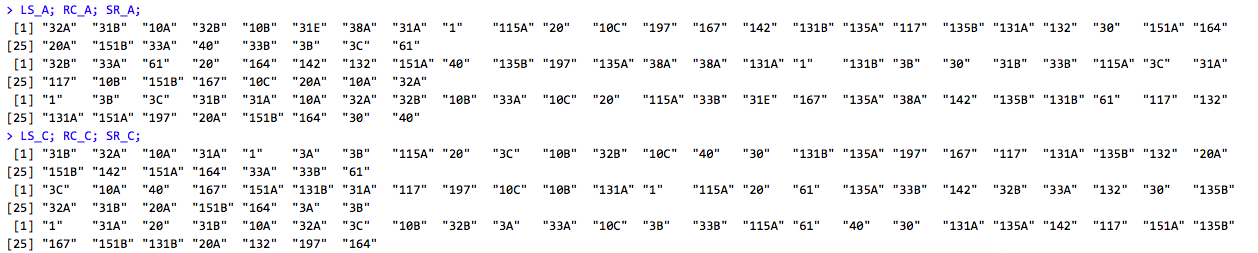
\includegraphics[width=6.5in]{rankings}
\caption{Rankings as computed by Least Squares (LS), Rank Centrality (RC), and Serial Rank (SR). Bucketed by GPA.}
\end{figure}

It can be hard to visualize how similar these rankings are, so we computed Kendall Tau Distances within each bucket:\\

\begin{verbatim}
  # for A bucket
  kendall_ls_sr_A <- kendall(LS_A, SR_A); # [1] 0.3004032
  kendall_ls_rc_A <- kendall(LS_A, RC_A); #
  kendall_rc_sr_A <- kendall(RC_A, SR_A); # [1] 0.3830645
  
  # for C bucket
  kendall_ls_sr_C <- kendall(LS_C, SR_C); # [1] 0.2365591
  kendall_ls_rc_C <- kendall(LS_C, RC_C); # [1] 0.5096774
  kendall_rc_sr_C <- kendall(RC_C, SR_C); # [1] 0.5870968
\end{verbatim}
\textcolor{white}{.}\\
Furthermore, to visualize how different the course orderings were for A and C students, we computed the Kendall Tau Distance for the Serial Ranking of these students, taking care to ensure that the comparison matrices only had courses common to all these students.\\

\begin{verbatim}
# find kendall distances between A and C buckets for each ranking
  commonCourses <- intersect(rownames(C_A), rownames(C_C));
  C_A_pruned <- matrixSubset(C_A, commonCourses);
  C_C_pruned <- matrixSubset(C_C, commonCourses);
  kendall_sr <- kendall(serialRank(C_A_pruned), serialRank(C_C_pruned));
\end{verbatim}
\textcolor{white}{.}\\
Which returns the value of 0.1862069 for \texttt{kendall\_sr}, illustrating that A and C students don't take courses in wildly different order, but that there does seem to be a consistent difference in their orderings.

\section{Summary and conclusion}  \label{sec:conclusion}
\subsection{DAG Construction}
Dishearteningly, once we constructed comparison matrices for students of A and C range GPA's, and then found the difference of these two matrices, we saw that there was little meaningful information to be had. This is to say, there were several entries with values that would suggest that a course should most definitely be taken before another course, but for which this distinction was not semantically meaningful. For example, the difference matrix suggested that PIC 10A somehow should be a prerequisite for Math 33B.\\

Our results may have been different if our data set was somehow even larger than it was, because the resulting buckets from divvying up students by GPA were rather small, which means the entries may have not been statistically significant and wrought with noise.\\

Moreover, such an analysis may have been more useful if the data we ran our algorithms on was somehow for a department lacking in prerequisites. That is to say, because the Math department enforces many sensical prerequisites, there were few if any students who took a very different ordering of courses than any other given student.

\subsection{Rank Centrality}
Our implementation for rank centrality sadly did not output a plausible ranking of courses as serial rank did. We believe the reason for this may be due to an incorrect choice of the eigenvector for $\pi$. $\pi$ is the top left eigenvector of the Probability matrix $P$ and the final assignment of courses to their scores. We assumed that the top left eigenvector is synonymous with the left eigenvector associated with the left eigenvalue of the highest magnitude (other than one). We came to this assumption after observing that this choice gave a more plausible ranking than other assumptions for the top left eigenvector. Although more plausible, the rankings we arrived with are still far from logical and must indicate error in our implementation of the algorithm.


\bibliographystyle{siam}

\end{pagewiselinenumbers}

\end{document}
